%-------------------------------------------------------------------------------
%	PACKAGES AND OTHER DOCUMENT CONFIGURATIONS
%-------------------------------------------------------------------------------

\documentclass{article}

\usepackage{fancyhdr} % Required for custom headers
\usepackage{lastpage} % Required to determine the last page for the footer
\usepackage{extramarks} % Required for headers and footers
\usepackage[usenames,dvipsnames]{color} % Required for custom colors
\usepackage{graphicx} % Required to insert images
\usepackage{listings} % Required for insertion of code
\usepackage{courier} % Required for the courier font
\usepackage{lipsum} % Used for inserting dummy 'Lorem ipsum' text
\usepackage{amsmath}
\pdfcompresslevel0

% ==============================================================================
% PYTHON
% ==============================================================================
\usepackage[utf8]{inputenc}

% Default fixed font does not support bold face
\DeclareFixedFont{\ttb}{T1}{txtt}{bx}{n}{12} % for bold
\DeclareFixedFont{\ttm}{T1}{txtt}{m}{n}{12}  % for normal

% Custom colors
\usepackage{color}
\definecolor{deepblue}{rgb}{0,0,0.5}
\definecolor{deepred}{rgb}{0.6,0,0}
\definecolor{deepgreen}{rgb}{0,0.5,0}

\usepackage{listings}

% Python style for highlighting
\newcommand\pythonstyle{\lstset{
language=Python,
basicstyle=\ttm,
otherkeywords={self},             % Add keywords here
keywordstyle=\ttb\color{deepblue},
emph={MyClass,__init__},          % Custom highlighting
emphstyle=\ttb\color{deepred},    % Custom highlighting style
stringstyle=\color{deepgreen},
frame=tb,                         % Any extra options here
showstringspaces=false,            % 
breaklines=true
}}


% Python environment
\lstnewenvironment{python}[1][]
{\pythonstyle\lstset{#1}
}
{}

% Python for external files
\newcommand\pythonexternal[2][]{{
\pythonstyle\lstinputlisting[#1]{#2}}}

% Python for inline
\newcommand\pythoninline[1]{{\pythonstyle\lstinline!#1!}}
% ==============================================================================
% ==============================================================================

% Margins
\topmargin=-0.45in
\evensidemargin=0in
\oddsidemargin=0in
\textwidth=6.5in
\textheight=9.0in
\headsep=0.25in

\linespread{1.1} % Line spacing

% Set up the header and footer
\pagestyle{fancy}
\lhead{\hmwkAuthorName} % Top left header
\chead{\hmwkClass\ (\hmwkClassInstructor\ \hmwkClassTime): \hmwkTitle} % Top center head
\rhead{\firstxmark} % Top right header
\lfoot{\lastxmark} % Bottom left footer
\cfoot{} % Bottom center footer
\rfoot{Page\ \thepage\ of\ \protect\pageref{LastPage}} % Bottom right footer
\renewcommand\headrulewidth{0.4pt} % Size of the header rule
\renewcommand\footrulewidth{0.4pt} % Size of the footer rule

\setlength\parindent{0pt} % Removes all indentation from paragraphs

%----------------------------------------------------------------------------------------
%	DOCUMENT STRUCTURE COMMANDS
%	Skip this unless you know what you're doing
%----------------------------------------------------------------------------------------

% Header and footer for when a page split occurs within a problem environment
\newcommand{\enterProblemHeader}[1]{\nobreak\extramarks{#1}{#1 continued on next page\ldots}\nobreak\nobreak\extramarks{#1 (continued)}{#1 continued on next page\ldots}\nobreak}

% Header and footer for when a page split occurs between problem environments
\newcommand{\exitProblemHeader}[1]{\nobreak\extramarks{#1 (continued)}{#1 continued on next page\ldots}\nobreak\nobreak\extramarks{#1}{}\nobreak}

\setcounter{secnumdepth}{0} % Removes default section numbers
\newcounter{homeworkProblemCounter} % Creates a counter to keep track of the number of problems

\newcommand{\homeworkProblemName}{}
\newenvironment{homeworkProblem}[1][Problem \arabic{homeworkProblemCounter}]{ % Makes a new environment called homeworkProblem which takes 1 argument (custom name) but the default is "Problem #"
\stepcounter{homeworkProblemCounter} % Increase counter for number of problems
\renewcommand{\homeworkProblemName}{#1} % Assign \homeworkProblemName the name of the problem
\section{\homeworkProblemName} % Make a section in the document with the custom problem count
\enterProblemHeader{\homeworkProblemName} % Header and footer within the environment
}{\exitProblemHeader{\homeworkProblemName} % Header and footer after the environment
}

% Defines the problem answer command with the content as the only argument
\newcommand{\problemAnswer}[1]{\noindent\framebox[\columnwidth, resolution=600][c]{\begin{minipage}{0.98\columnwidth, resolution=600}#1\end{minipage}}}
% Makes the box around the problem answer and puts the content inside }

\newcommand{\homeworkSectionName}{}
\newenvironment{homeworkSection}[1]{ % New environment for sections within homework problems, takes 1 argument - the name of the section
\renewcommand{\homeworkSectionName}{#1} % Assign \homeworkSectionName to the name of the section from the environment argument
\subsection{\homeworkSectionName} % Make a subsection with the custom name of the subsection
\enterProblemHeader{\homeworkProblemName\ [\homeworkSectionName]} % Header and footer within the environment
}{
\enterProblemHeader{\homeworkProblemName} % Header and footer after the environment
}

%----------------------------------------------------------------------------------------
%	NAME AND CLASS SECTION
%----------------------------------------------------------------------------------------

\newcommand{\hmwkTitle}{Homework 3} % Assignment title
\newcommand{\hmwkDueDate}{Friday, April 4} % Due date
\newcommand{\hmwkClass}{Astron 730} % Course/class
\newcommand{\hmwkClassTime}{2:25 pm} % Class/lecture time
\newcommand{\hmwkClassInstructor}{Tremonti} % Teacher/lecturer
\newcommand{\hmwkAuthorName}{Elijah Bernstein-Cooper} % Your name

%-------------------------------------------------------------------------------
%	TITLE PAGE
%-------------------------------------------------------------------------------

\title{\vspace{2in}
    \textmd{\textbf{\hmwkClass:\ \hmwkTitle}}\\
    \normalsize\vspace{0.1in}\small{Due\ on\ \hmwkDueDate}\\
    \vspace{0.1in}\large{\textit{\hmwkClassInstructor\ \hmwkClassTime}}
    \vspace{3in}}

\author{\textbf{Elijah Bernstein-Cooper}}
\date{\today} % Insert date here if you want it to appear below your name

%-------------------------------------------------------------------------------

\begin{document}

\maketitle
\newpage

%===============================================================================
%-------------------------------------------------------------------------------
%	PROBLEM 1
%-------------------------------------------------------------------------------
\begin{homeworkProblem}
    %---------------------------------------------------------------------------
    %	PROBLEM 1a
    %---------------------------------------------------------------------------
    \begin{homeworkSection}{1a}

        %-----------------------------------------------------------------------
        % FIGURE
        \begin{figure}[!ht]
        \begin{center}
            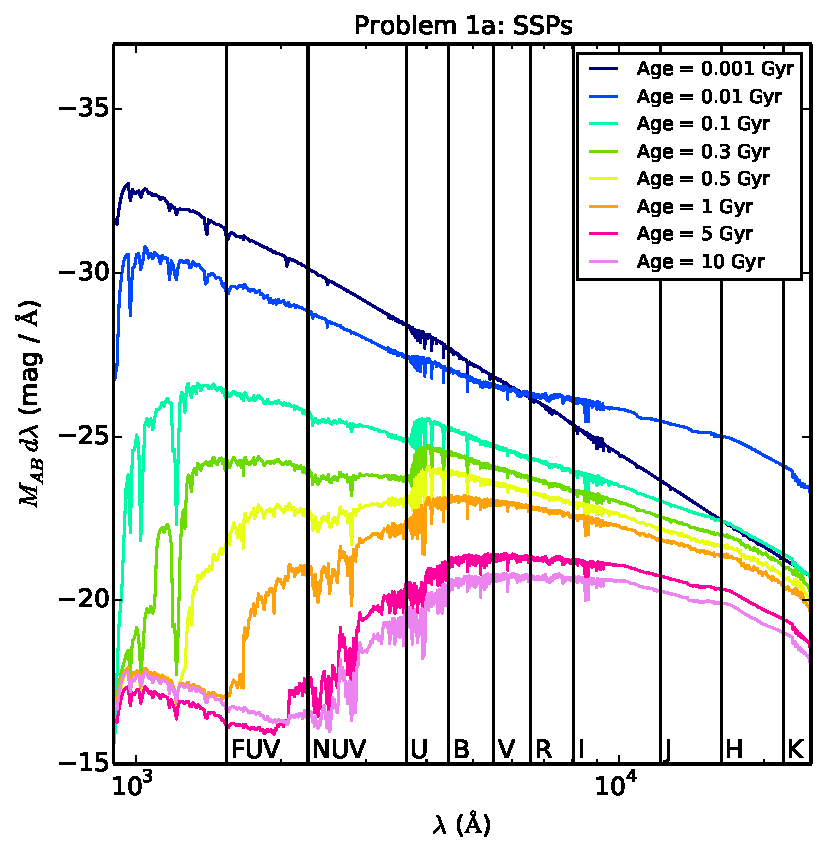
\includegraphics[width=1\columnwidth]{p_1a.pdf} 

            \caption{\label{fig:1a} SSPs with ages of approximately 0.001,
            0.01, 0.1, 0.3, 0.5, 1, 5, and 10 Gyr. The centers of the UBVRIJHK
            filters and the GALEX FUV and NUV filters are labeled as well.
            These SSP absolute magnitudes were derived from 1 $M_\odot$ of
            stars with a perfectly sampled Chabrier IMF.}

        \end{center}
        \end{figure}
        %-----------------------------------------------------------------------
    
    \end{homeworkSection}

    %---------------------------------------------------------------------------
    %	PROBLEM 1b
    %---------------------------------------------------------------------------
    \begin{homeworkSection}{1b}

        %-----------------------------------------------------------------------
        % FIGURE
        \begin{figure}[!ht]
        \begin{center}
            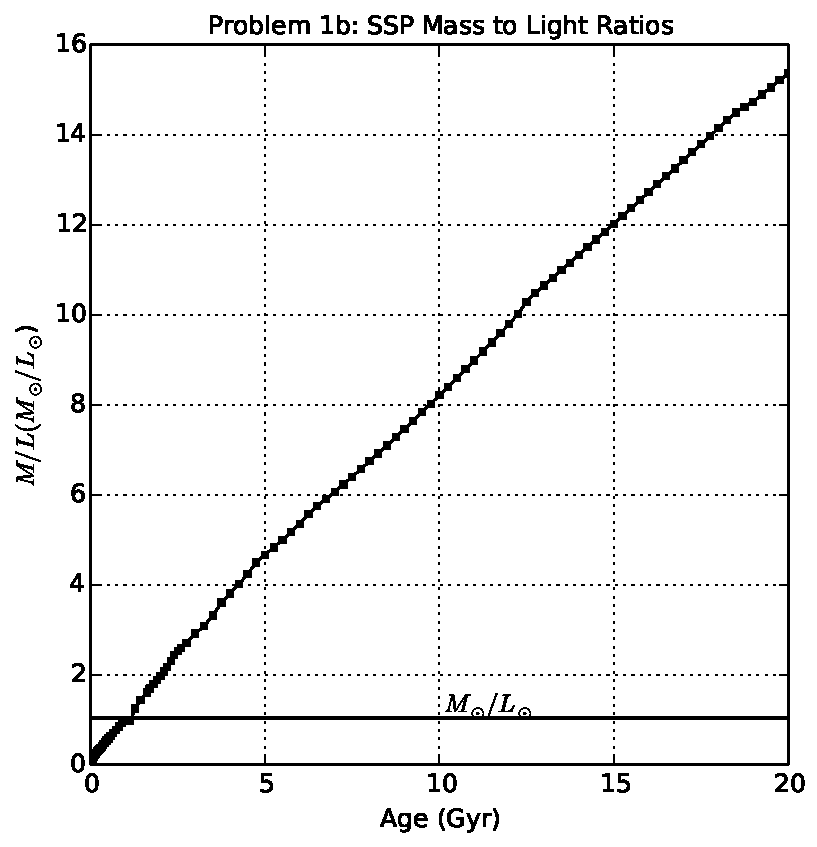
\includegraphics[width=1\columnwidth]{p_1b.pdf} 

            \caption{\label{fig:1b} The mass-to-light (M/L) ratio at 5500$\AA$
            as a function of stellar population age. For reference, the solar
            mass to light ratio in the $V$-band is shown.}

        \end{center}
        \end{figure}
        %-----------------------------------------------------------------------
    
    \end{homeworkSection}
    
    %---------------------------------------------------------------------------
    %	PROBLEM 1c
    %---------------------------------------------------------------------------
    \begin{homeworkSection}{1c}

        %-----------------------------------------------------------------------
        % FIGURE
        \begin{figure}[!ht]
        \begin{center}
            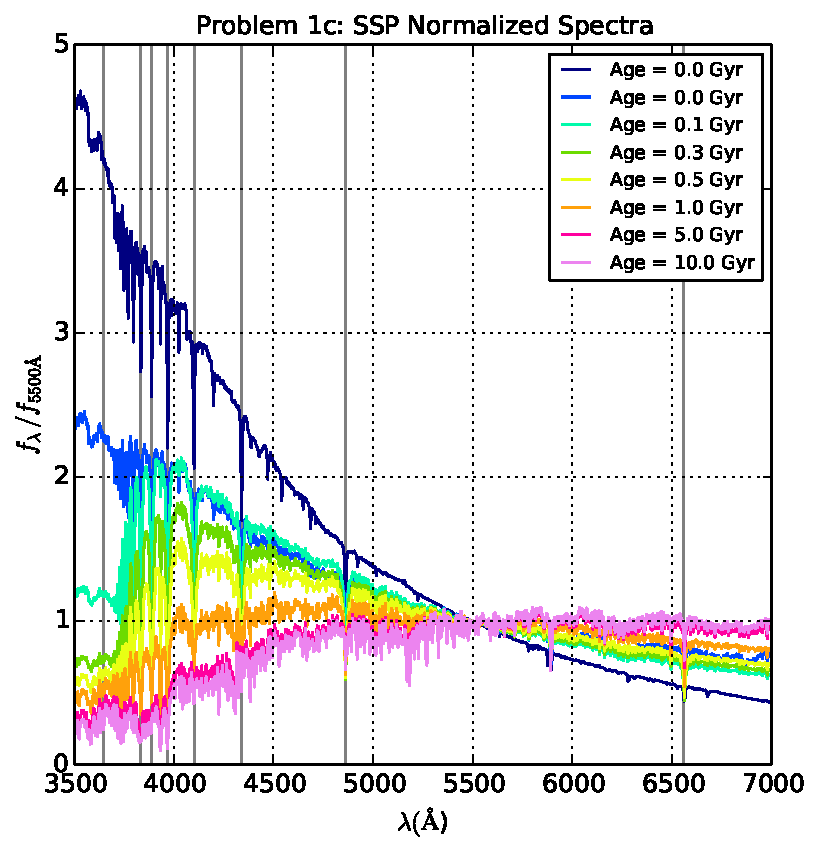
\includegraphics[width=1\columnwidth]{p_1c.pdf} 

            \caption{\label{fig:1c} Same as Figure~\ref{fig:1a} except the
            normalized fluxes of each star are plotted. The faint gray lines
            represent the locations of Balmer absorption lines. Balmer
            absorption lines are strongest at younger ages in these SSP.}

        \end{center}
        \end{figure}
        %-----------------------------------------------------------------------
    
    \end{homeworkSection}
\end{homeworkProblem}
\clearpage
%===============================================================================



%===============================================================================
%-------------------------------------------------------------------------------
%	PROBLEM 2
%-------------------------------------------------------------------------------
\begin{homeworkProblem}
    %---------------------------------------------------------------------------
    %	PROBLEM 2a
    %---------------------------------------------------------------------------
    \begin{homeworkSection}{2a}

        %-----------------------------------------------------------------------
        % FIGURE
        \begin{figure}[!ht]
        \begin{center}
            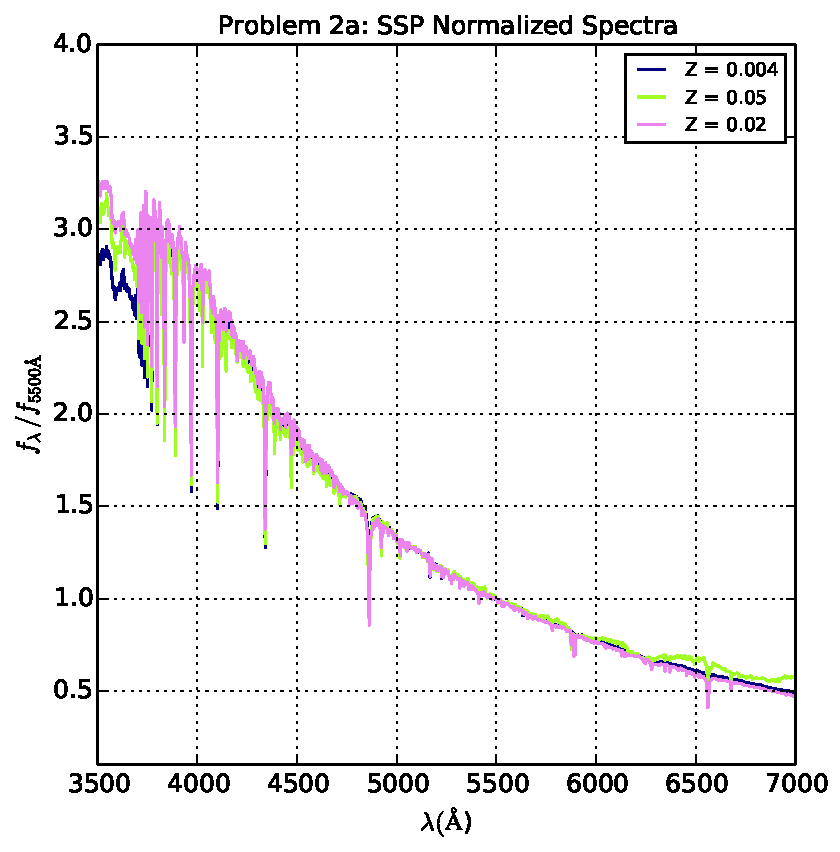
\includegraphics[width=1\columnwidth]{p_2a.pdf} 

            \caption{\label{fig:2a} 5 Myr old spectra for three different
            SSPs with varying metallicities, flux-normalized at 5500 $\AA$.}

        \end{center}
        \end{figure}
        %-----------------------------------------------------------------------
    \end{homeworkSection}
    
    %---------------------------------------------------------------------------
    %	PROBLEM 2b
    %---------------------------------------------------------------------------
    \begin{homeworkSection}{2b}

        %-----------------------------------------------------------------------
        % FIGURE
        \begin{figure}[!ht]
        \begin{center}
            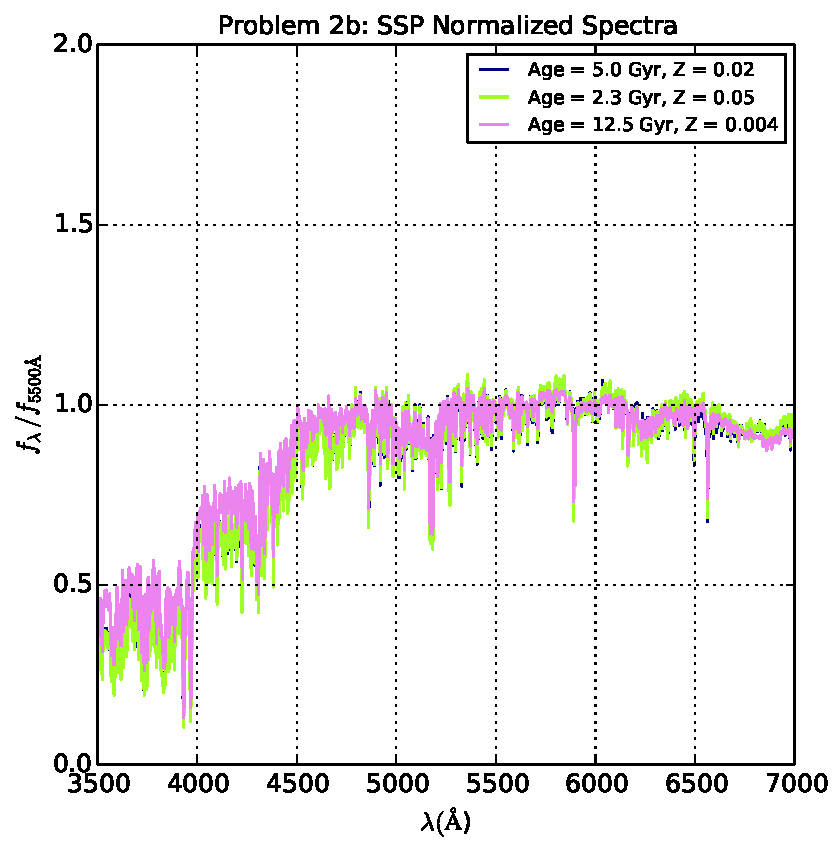
\includegraphics[width=1\columnwidth]{p_2b.pdf} 

            \caption{\label{fig:2b} 5 Myr old spectrum for solar metallicity
            SSP, flux-normalized at 5500 $\AA$. The best-fitting spectra of
            different ages over the range 3500--7000 $\AA$ of 0.004 and 0.05
            solar metallicity are plotted. The average residual between solar
            metallicity 5 Myr-old spectrum and the other spectrum for 0.004 and
            0.05 solar metallicity spectra over all ages is $< 1\%$.}

        \end{center}
        \end{figure}
        %-----------------------------------------------------------------------
    \end{homeworkSection}
    
    %---------------------------------------------------------------------------
    %	PROBLEM 2c
    %---------------------------------------------------------------------------
    \begin{homeworkSection}{2c}

        %-----------------------------------------------------------------------
        % FIGURE
        \begin{figure}[!ht]
        \begin{center}
            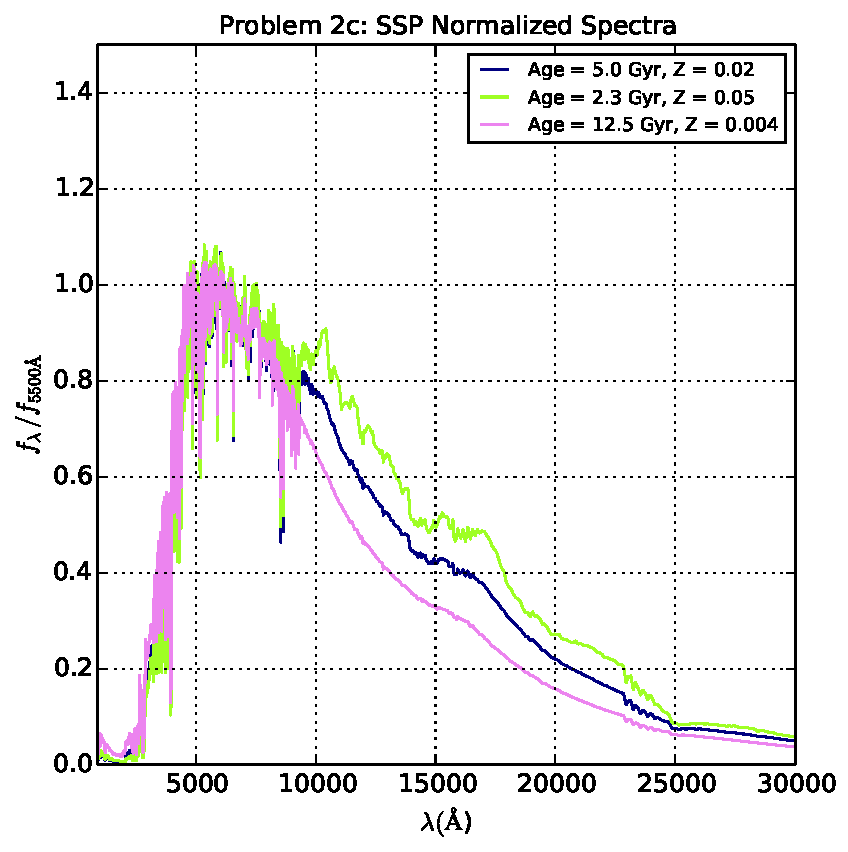
\includegraphics[width=1\columnwidth]{p_2c.pdf} 

            \caption{\label{fig:2c} Same as Figure~\ref{fig:2b} except over a
            different wavelength range. The best wavelengths to observe without
            an age-metallicity degeneracy are between 1$\mu m$ and 25$\mu m$.
            Unfortunately Red Giant Branch and Horizontal Branch stars outshine
            all other stars in these bands by orders of magnitudes, making the
            observation of MS stars difficult.}

        \end{center}
        \end{figure}
        %-----------------------------------------------------------------------
    \end{homeworkSection}
\end{homeworkProblem}
\clearpage

%===============================================================================

%===============================================================================
%-------------------------------------------------------------------------------
%	PROBLEM 3
%-------------------------------------------------------------------------------
\begin{homeworkProblem}
    %---------------------------------------------------------------------------
    %	PROBLEM 3a
    %---------------------------------------------------------------------------
    \begin{homeworkSection}{3a}

        %-----------------------------------------------------------------------
        % FIGURE
        \begin{figure}[!ht]
        \begin{center}
            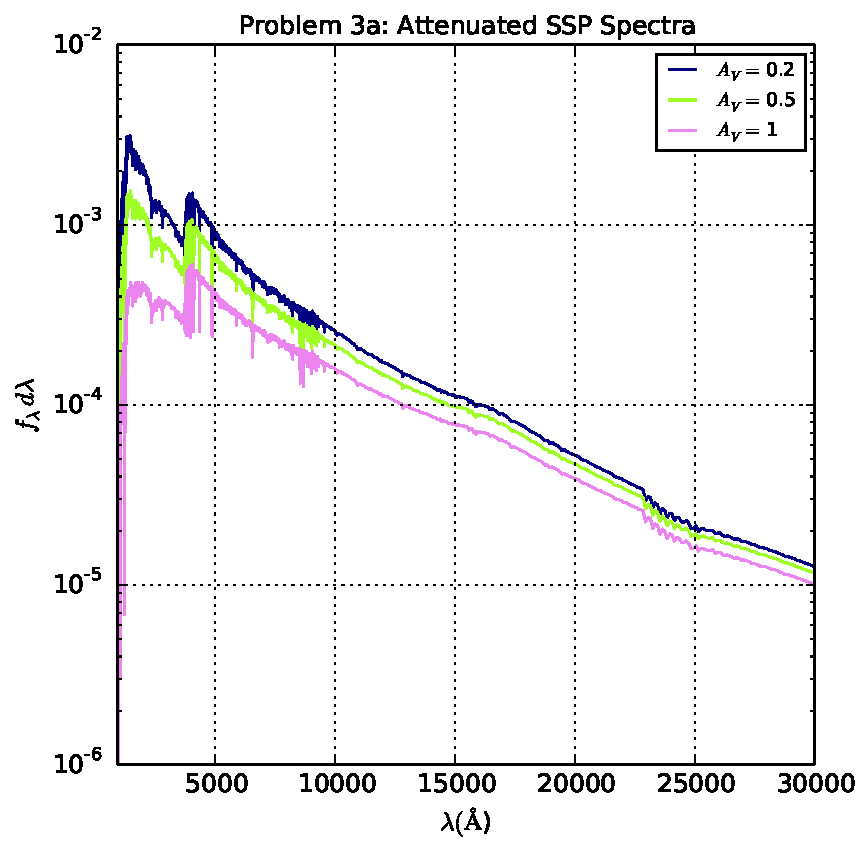
\includegraphics[width=1\columnwidth]{p_3a.pdf} 

            \caption{\label{fig:3a} 100 Myr-old solar metallicity model spectra
            with different $V$-band attenuation values.}

        \end{center}
        \end{figure}
        %-----------------------------------------------------------------------
    \end{homeworkSection}
    
    %---------------------------------------------------------------------------
    %	PROBLEM 3b
    %---------------------------------------------------------------------------
    \begin{homeworkSection}{3b}

        %-----------------------------------------------------------------------
        % FIGURE
        \begin{figure}[!ht]
        \begin{center}
            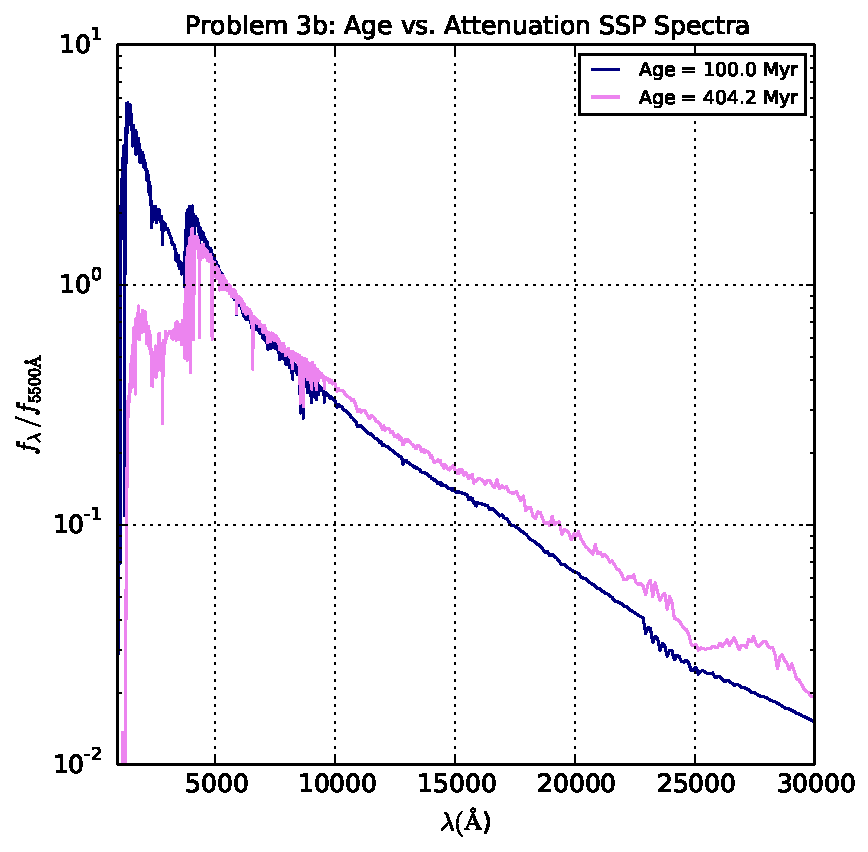
\includegraphics[width=1\columnwidth]{p_3b.pdf} 

            \caption{\label{fig:3b} Spectra of dust-free models with different
            metallicities and ages that best fit the 100 Myr old model with
            $A_V$ = 0.5 mag.  The fit was optimized over 3500--7000 $\AA$.
            Wavelengths between 1000 $\AA$ and 4,000 $\AA$ provide the best
            leverage for determining age vs.\ dust attenuation.}

        \end{center}
        \end{figure}
        %-----------------------------------------------------------------------
    \end{homeworkSection}
\end{homeworkProblem}
\clearpage
%===============================================================================

%===============================================================================
%-------------------------------------------------------------------------------
%	PROBLEM 4
%-------------------------------------------------------------------------------
\begin{homeworkProblem}
    %---------------------------------------------------------------------------
    %	PROBLEM 4a
    %---------------------------------------------------------------------------
    \begin{homeworkSection}{4a}

        %-----------------------------------------------------------------------
        % FIGURE
        \begin{figure}[!ht]
        \begin{center}
            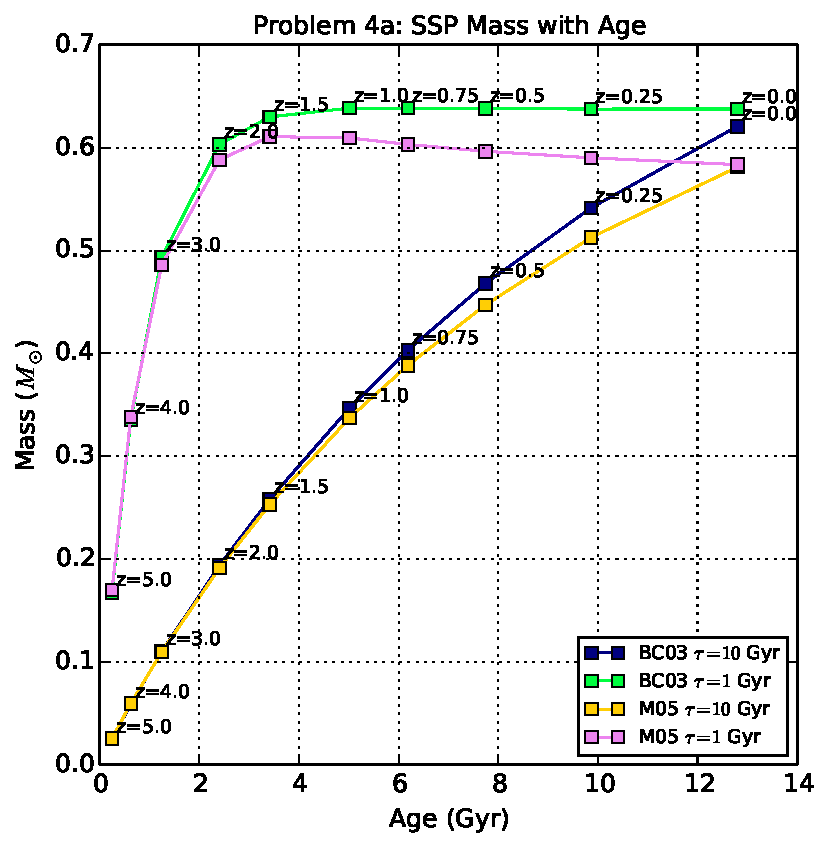
\includegraphics[width=1\columnwidth]{p_4a.pdf} 

            \caption{\label{fig:4a} Evolution of stellar mass versus age for
            all four of the models. The redshifts of the BC03 data are
            annotated.}

        \end{center}
        \end{figure}
        %-----------------------------------------------------------------------
    \end{homeworkSection}
    
    %---------------------------------------------------------------------------
    %	PROBLEM 4b
    %---------------------------------------------------------------------------
    \begin{homeworkSection}{4b}

        %-----------------------------------------------------------------------
        % FIGURE
        \begin{figure}[!ht]
        \begin{center}
            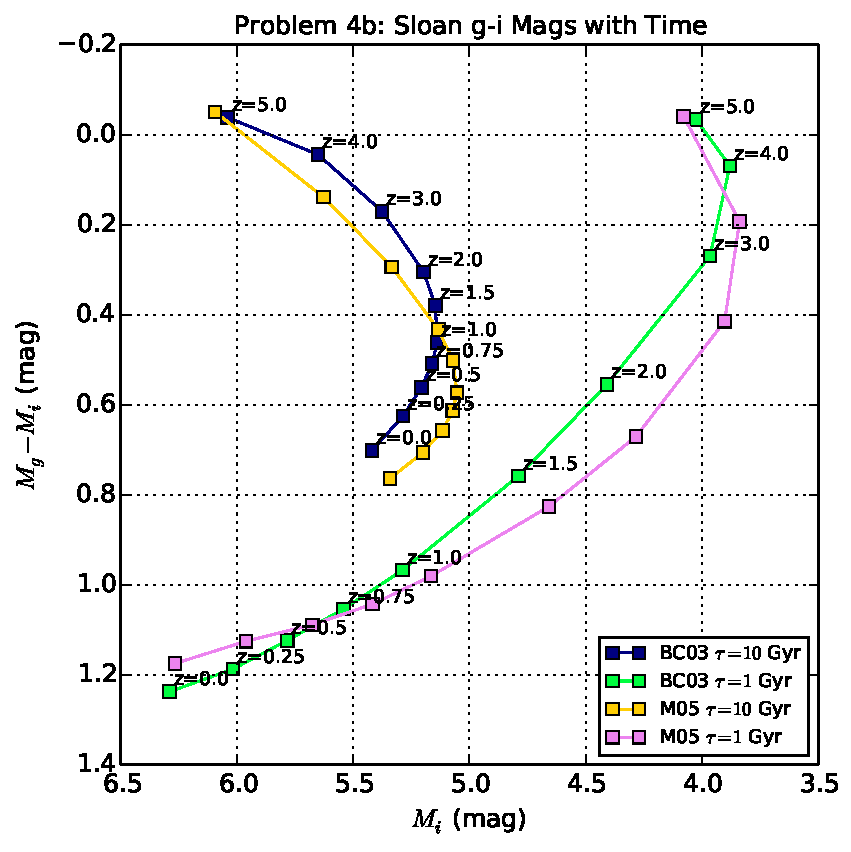
\includegraphics[width=1\columnwidth]{p_4b.pdf} 

            \caption{\label{fig:4b} Evolution of  $(g - i)$ vs.\ $i$ color
            magnitudes for all four of the models. The redshifts of the BC03
            data are annotated. We see an increase of $i$ magnitude then a
            decrease with time. This is due to more massive stars moving to the
            red giant branch, where they are very luminous in the NIR, but soon
            die, leaving the older stellar population whose spectra peak in the
            IR.}

        \end{center}
        \end{figure}
        %-----------------------------------------------------------------------
    \end{homeworkSection}
    
    %---------------------------------------------------------------------------
    %	PROBLEM 4c
    %---------------------------------------------------------------------------
    \begin{homeworkSection}{4c}

        The mass-to-light ratios must be conserved in this merger. We will
        determine the mass ratio needed of a late-type and an early-type
        galaxy where the merging galaxies are 13 Gyr old and produce a
        merged galaxy with a color of a 8 Gyr old early-type galaxy. Thus we
        define the following:

        \begin{itemize}
            \item $F_{e,10}$ is the flux of the 10-Gyr old early-type galaxy.
            \item $F_{l,10}$ is the flux of the 10-Gyr old late-type galaxy.
            \item $F_{e,5}$ is the flux of the 5-Gyr old early-type galaxy.
            \item $M_{e,10}$ is the mass of the 10-Gyr old early-type galaxy.
            \item $M_{l,10}$ is the mass of the 10-Gyr old late-type galaxy.
            \item $M_{e,5} = M_{e,10} + M_{l,10}$ is the mass of the 5-Gyr old early-type galaxy.
        \end{itemize}

        The conserved mass-to-light ratio will be

        \begin{equation}
            \frac{M_{e,10}}{F_{e,10}} + \frac{M_{l,10}}{F_{l,10}} =
            \frac{M_{e,5}}{F_{e,5}}
        \end{equation} 

        \noindent assigning $\alpha = M_{e,10} / M_{l,10}$, and substituting
        for $M_{l,10}$

        \begin{equation}
            \frac{1}{F_{e,10}} + \frac{1}{\alpha F_{l,10}} =
            \frac{1 + \frac{1}{\alpha}}{F_{e,5}}
        \end{equation}

        \begin{equation}
            \alpha = \frac{F_{e,5}^{-1} - F_{l,10}^{-1}}
                          {F_{e,10}^{-1} - F_{e,5}^{-1}}
        \end{equation}

        For colors we will have

        \begin{equation}
            (\frac{M_{e,10,g}}{F_{e,10,g}} - \frac{M_{e,10,i}}{F_{e,10,i}}) +
            (\frac{M_{l,10,g}}{F_{l,10,g}} - \frac{M_{l,10,i}}{F_{l,10,i}})
            =
            \frac{M_{e,5,i}}{F_{e,5,i}} - \frac{M_{e,5,i}}{F_{e,5,i}}
        \end{equation} 

        \begin{equation}
            M_{e,10,g} (\frac{1}{F_{e,10,g}} - \frac{1}{F_{e,10,i}}) + 
            M_{l,10,g} (\frac{1}{F_{l,10,g}} - \frac{1}{F_{l,10,i}})
            =
            M_{e,5,i} (\frac{1}{F_{e,5,i}} - \frac{1}{F_{e,5,i}})
        \end{equation} 

        \noindent and using similar steps as above we arrive at

        \begin{equation}
            \alpha = \frac{(F_{e,5,g}^{-1} - F_{e,5,i}^{-1}) - 
                                (F_{l,10,g}^{-1} - F_{l,10,i}^{-1})}
                          {(F_{e,10,g}^{-1} - F_{e,10,i}^{-1}) - 
                                (F_{e,5,g}^{-1} - F_{e,5,i}^{-1})}
        \end{equation}

        Thus the mass ratio needed for a merging late-type and
        early-type galaxy 13 Gyr old to reproduce the color of a 8 Gyr old
        early-type galaxy is

        \begin{equation}
            \frac{M_{e,10}}{M_{l,10}} = 3.87
        \end{equation}

    \end{homeworkSection}

        
\end{homeworkProblem}
\clearpage
%===============================================================================

\end{document}

